\documentclass[article]{jss}

%% -- LaTeX packages and custom commands ---------------------------------------

%% recommended packages
\usepackage{thumbpdf,lmodern}

%% additional packages
\usepackage{amssymb,amsmath}

%% new custom commands
\newcommand{\class}[1]{`\code{#1}'}
\newcommand{\fct}[1]{\code{#1()}}

%% For Sweave-based articles about R packages:
%% need no \usepackage{Sweave}



%% -- Article metainformation (author, title, ...) -----------------------------

%% - \author{} with primary affiliation
%% - \Plainauthor{} without affiliations
%% - Separate authors by \And or \AND (in \author) or by comma (in \Plainauthor).
%% - \AND starts a new line, \And does not.
\author{Lennart Oelschl\"ager \\Bielefeld University \And Timo Adam \\University of St Andrews\And Rouven Michels \\Bielefeld University}
\Plainauthor{Lennart Oelschl\"ager, Timo Adam, Rouven Michels}

%% - \title{} in title case
%% - \Plaintitle{} without LaTeX markup (if any)
%% - \Shorttitle{} with LaTeX markup (if any), used as running title
\title{\pkg{fHMM}: Hidden Markov Models for Financial Time Series in \proglang{R}}
\Plaintitle{fHMM: Hidden Markov Models for Financial Time Series in R}
\Shorttitle{fHMM}

%% - \Abstract{} almost as usual
\Abstract{
Hidden Markov models constitute a popular class of statistical models for time series that are driven by hidden states. In finance, these hidden states can often be linked to market regimes such as bearish and bullish markets or recessions and periods of economics growths, to name but a few examples. Hidden Markov models account for these state-switching patterns by... In this paper, we introduce the \proglang{R} package \pkg{fHMM} that provides various tools for modeling financial time series using hidden Markov models. Its key features include...
}

%% - \Keywords{} with LaTeX markup, at least one required
%% - \Plainkeywords{} without LaTeX markup (if necessary)
%% - Should be comma-separated and in sentence case.
\Keywords{decoding market behavior, hidden Markov models, time series modeling, \proglang{R}}
\Plainkeywords{decoding market behavior, hidden Markov models, time series modeling, R}

%% - \Address{} of at least one author
%% - May contain multiple affiliations for each author
%%   (in extra lines, separated by \emph{and}\\).
%% - May contain multiple authors for the same affiliation
%%   (in the same first line, separated by comma).
\Address{
  Lennart Oelschl\"ager\\
  Department of Business Administration and Economics\\
  Bielefeld University\\
  Postfach 10 01 31\\
  E-mail: \email{lennart.oelschlaeger@uni-bielefeld.de}
}

\begin{document}
%% Do we need to following line?
%% \SweaveOpts{concordance=TRUE}

%% -- Introduction -------------------------------------------------------------

%% - In principle "as usual".
%% - But should typically have some discussion of both _software_ and _methods_.
%% - Use \proglang{}, \pkg{}, \fct{} and \code{} markup throughout the manuscript.
%% - If such markup is in (sub)section titles, a plain text version has to be
%%   added as well.
%% - All software mentioned should be properly \cite-d.
%% - All abbreviations should be introduced.
%% - Unless the expansions of abbreviations are proper names (like "Journal
%%   of Statistical Software" above) they should be in sentence case (like
%%   "generalized linear models" below).

\section{Introduction}
\label{sec:intro} %% Timo 

%% Earning money with stock trading is simple: one only needs to buy and sell stocks at the right moment. In general, stock traders seek to invest at the beginning of upward trends (hereon termed as bullish markets) and repel their stocks just in time before the prices fall again (hereon termed as bearish markets). As stock prices depend on a variety of environmental factors \cite{hum09}, \cite{coh13}, chance certainly plays a fundamental role in hitting those exact moments. However, investigating market behavior can lead to a better understanding of how trends alternate and thereby increases the chance of making profitable investment decisions. 

%% Intro to HMMs
In recent years, hidden Markov models (HMMs) have emerged as a popular tool for modeling time series that are subject to state-switching over time \citep{zuc16}. In their basic form, HMMs comprise an observed state-dependent process that is driven by a hidden state process, the latter of which is typically modeled using a discrete-time, finite-state Markov chain. In financial applications, the states of the underlying Markov chain can often be linked to market regimes such as bearish and bullish markets or recessions and periods of economics growths: when the market is in a calm state, then the observations follow some distribution, whereas when the market is in a nervous state, then another distribution is active to generate the observations. By their dependence structure, HMMs naturally account for such state-switching patterns and thus allow us to infer hidden market regimes and their dynamics from financial time series.

%% Literature review
Over the last decades, HMMs have been applied to various financial problems, including modeling business cycles \cite{gre00}, deriving stylized facts of stock returns \cite{bul06, nys15a}, and modeling energy prices conditional on market regimes \cite{lan18, ada22}, to name but a few examples.
More recently, \cite{lih17} used HMMs to identify different volatility levels in the Standard and Poor's 500 index, aiming at providing evidence for the conjecture that returns exhibit negative correlation with volatility. \cite{ngu18}, to give another example, used HMMs to predict monthly closing prices to derive an optimal trading strategy, which was shown to outperform the conventional buy-and-hold strategy. Further financial applications include HMMs for asset allocation and portfolio optimization \citep{bul11, nys15a, nys18}. All these examples demonstrate that HMMs constitute a versatile class of time series models that naturally accounts for the state-switching patterns that are often found in financial time series.

%% Intro to the package
The \pkg{fHMM} package aims at making HMMs accessible to users interested in modeling financial time series. Its functionality can be classified into functions for data preparation, model estimation, and model evaluation, which is illustrated in Figure \ref{fig:flowchart}. Functions for data preparation include an interface to Yahoo Finance... The model is estimated in a maximum likelihood framework, where the likelihood is evaluated using the forward algorithm, which is implemented in C++. Functions for model evaluation include... It also implements hierarchical HMMs; an extension of basic HMMs proposed in \cite{oel21} that improves the model's capability of distinguishing between short- and long-term trends and allows us to model data collected at different time scales. interpret market dynamics at multiple time scales. 

\begin{figure}
  \centering
  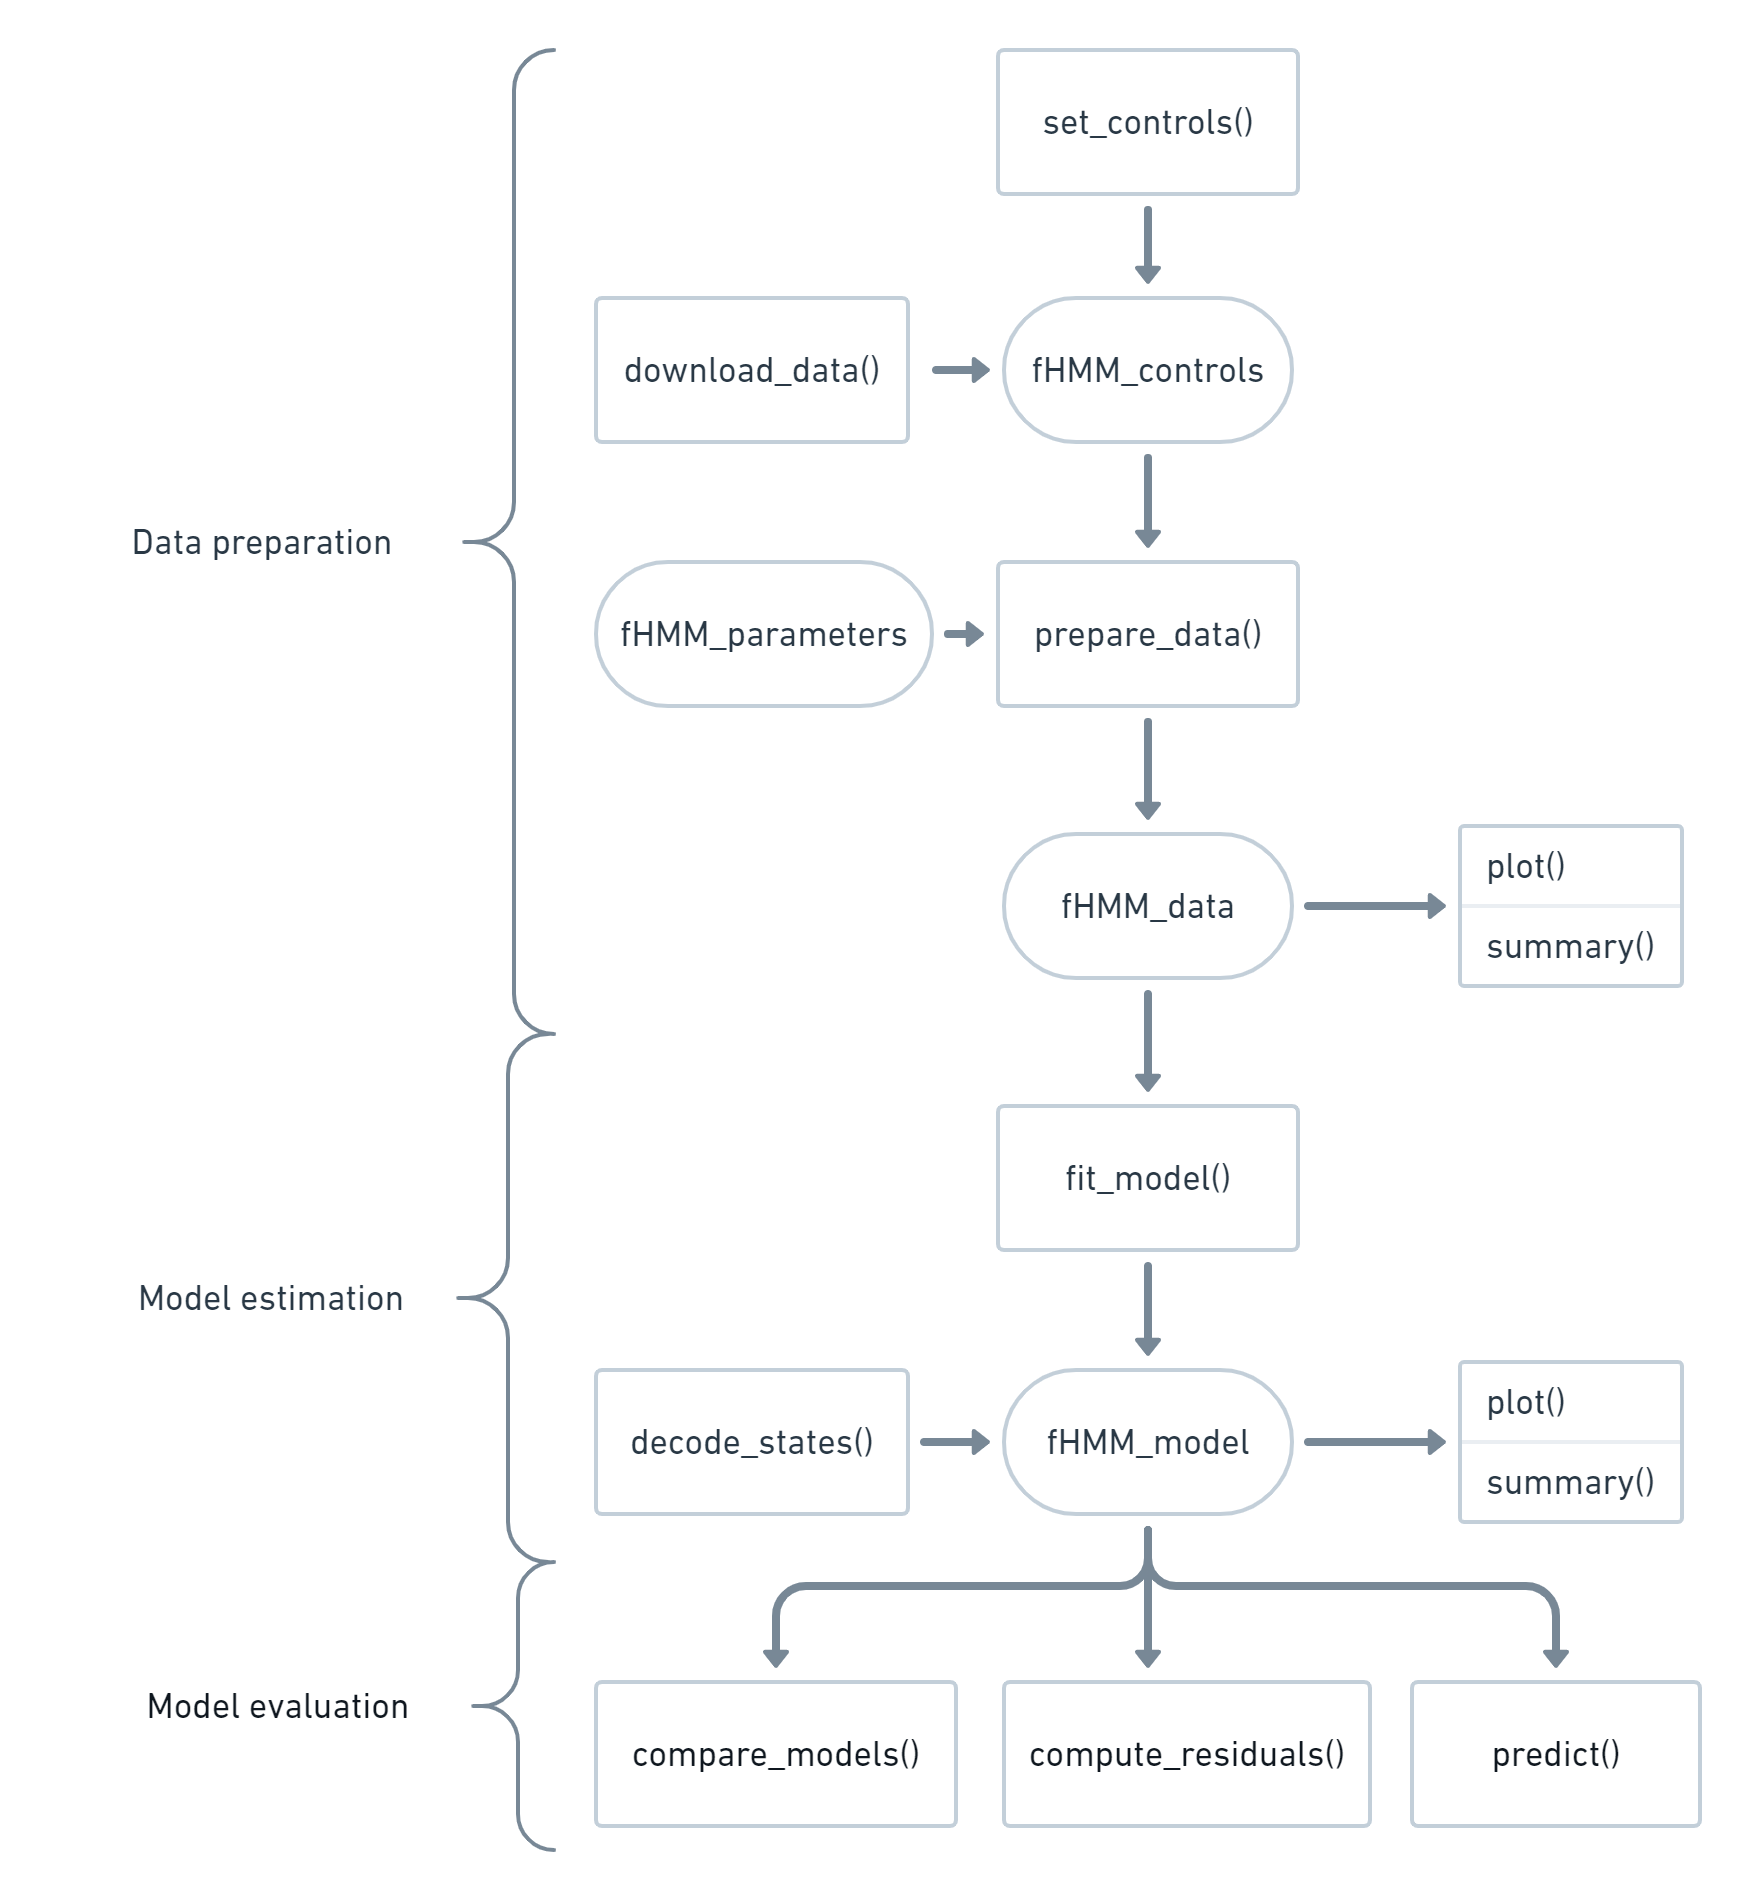
\includegraphics[scale = 0.4]{flowchart.png}
  \caption{Flowchart of the package functionality.}
  \label{fig:flowchart}
\end{figure}

%% Outline of the paper
This paper is structured as follows: in Section 2, ... In Section 3, ...

%% -- Manuscript ---------------------------------------------------------------

%% - In principle "as usual" again.
%% - When using equations (e.g., {equation}, {eqnarray}, {align}, etc.
%%   avoid empty lines before and after the equation (which would signal a new
%%   paragraph.
%% - When describing longer chunks of code that are _not_ meant for execution
%%   (e.g., a function synopsis or list of arguments), the environment {Code}
%%   is recommended. Alternatively, a plain {verbatim} can also be used.
%%   (For executed code see the next section.)
%% - Tables are placed at the top of the page
%%   (\verb|[t!]|), centered (\verb|\centering|), with a caption below the table,
%%   column headers and captions in sentence style, and if possible avoiding
%%   vertical lines.
%% - Virtually all JSS manuscripts list source code along with the generated
%%   output. The style files provide dedicated environments for this.
%% - In R, the environments {Sinput} and {Soutput} - as produced by Sweave() or
%%   or knitr using the render_sweave() hook - are used (without the need to
%%   load Sweave.sty).
%% - Equivalently, {CodeInput} and {CodeOutput} can be used.
%% - The code input should use "the usual" command prompt in the respective
%%   software system.
%% - For R code, the prompt "R> " should be used with "+  " as the
%%   continuation prompt.
%% - Comments within the code chunks should be avoided - these should be made
%%   within the regular LaTeX text.
%% - Please make sure that all code is properly spaced, e.g., using
%%   \code{y = a + b * x} and \emph{not} \code{y=a+b*x}.
%% - JSS prefers when the second line of code is indented by two spaces.

\section{Model definition} \label{sec:model_definition} %% Rouven

Hidden Markov models (HMMs) are a modeling framework for time series data where a sequence of observation is assumed to depend on a latent state process. The peculiarity is that, instead of the observation process, the state process cannot be directly observed. However, the latent states comprise information about the environment the model is applied on. 

The connection between hidden state process and observed state-dependent process arises by the following: Let $N$ be the number of possible states. We assume that for each point in time $t = 1, \ldots, T$, an underlying process $(S_t)_{t = 1, \ldots, T}$ is in one of those $N$ states. Then, depending on the active state $S_t \in \{ 1, \ldots, N \}$, the observation $X_t$ from the state-dependent process $(X_t)_{t = 1, \ldots, T}$ is assumed to be generated by the corresponding distribution of the $N$ distributions $f^{(1)},\dots,f^{(N)}.$

Furthermore, we assume $(S_t)_t$ to be Markovian, i.e.\ we assume that the actual state only depends on the previous state. Henceforth, we can identify the process by its initial distribution $\delta$ and its transition probability matrix (t.p.m.) $\Gamma$. Moreover, by construction, we force the process $(X_t)_{t = 1, \ldots, T}$ to satisfy the conditional independence assumption, i.e.\ the actual observation $X_t$ depends on the current state $S_t$, but does not depend on previous observations or states at all.

Referring to financial data, the different states can serve as proxies for the actual market situation, e.g. calm or nervous. Even though these moods cannot be observed directly, price changes or trading volumes, which clearly depend on the current mood of the market, can be observed. Thereby, using an underlying Markov process, we can detect which mood is active at any point in time and how the different moods alternate. Depending on the current mood, a price change is generated by a different distribution. These distributions characterize the moods in terms of expected return and volatility. For example, we can model price changes at time point $t$ to be generated by different normal distributions whose mean and volatility depend on $S_t$.

Following \cite{zuc16}, we assume that the initial distribution $\delta$ equals the stationary distribution $\pi$, where $\pi = \pi \Gamma$, i.e.\ the stationary and henceforth the initial distribution is determined by $\Gamma$. If the Markov process is irreducible, it has a unique distribution, which solves $\pi = \pi \Gamma$. If
additionally the Markov process is aperiodic, its state distribution converges to the stationary distribution, see \cite{nor97}. Irreducibility and aperiodicity are usually satisfied assumptions in reality. This is reasonable from a practical point of view: On the one hand, the hidden state process has been evolving for some time before we start to observe it and hence can be assumed to be stationary. On the other hand, setting $\delta=\pi$ reduces the number of parameters that need to be estimated, which is convenient from a computational perspective.

The hierarchical hidden Markov model (HMMM) is a flexible extension of the HMM  that can jointly model data observed on two different time scales. The two time series, one on a coarser and one on a finer scale, differ in the number of observations, e.g. monthly observations on the coarser scale and daily or weekly observations on the finer scale. 

Following the concept of HMMs, we can model both state-dependent time series jointly. First, we treat the time series on the coarser scale as stemming from an ordinary HMM, which we refer to as the coarse-scale HMM: At each time point $t$ of the coarse-scale time space $\{1,\dots,T\}$, an underlying process $(S_t)_t$ selects one state from the coarse-scale state space $\{1,\dots,N\}$. We call $(S_t)_t$ the hidden coarse-scale state process. Depending on which state is active at $t$, one of $N$ distributions $f^{(1)},\dots,f^{(N)}$ realizes the observation $X_t$. The process $(X_t)_t$ is called the observed coarse-scale state-dependent process. The processes $(S_t)_t$ and $(X_t)_t$ have the same properties as before, namely $(S_t)_t$ is a first-order Markov process and $(X_t)_t$ satisfies the conditional independence assumption. 

Subsequently, we segment the observations of the fine-scale time series into $T$ distinct chunks, each of which contains all data points that correspond to the $t$-th coarse-scale time point. Assuming that we have $T^*$ fine-scale observations on every coarse-scale time point, we face $T$ chunks comprising of $T^*$ fine-scale observations each. 

The hierarchical structure now evinces itself as we model each of the chunks by one of $N$ possible fine-scale HMMs. Each of the fine-scale HMMs has its own t.p.m.\ $\Gamma^{*(i)}$, initial distribution $\delta^{*(i)}$, stationary distribution $\pi^{*(i)}$, and state-dependent distributions $f^{*(i,1)},\dots,f^{*(i,N^*)}$. Which fine-scale HMM is selected to explain the $t$-th chunk of fine-scale observations depends on the hidden coarse-scale state $S_t$. The $i$-th fine-scale HMM explaining the $t$-th chunk of fine-scale observations consists of the following two stochastic processes: At each time point $t^*$ of the fine-scale time space $\{1,\dots,T^*\}$, the process $(S^*_{t,t^*})_{t^*}$ selects one state from the fine-scale state space $\{1,\dots,N^*\}$. We call $(S^*_{t,t^*})_{t^*}$ the hidden fine-scale state process. Depending on which state is active at $t^*$, one of $N^*$ distributions $f^{*(i,1)},\dots,f^{*(i,N^*)}$ realizes the observation $X^*_{t,t^*}$. The process $(X^*_{t,t^*})_{t^*}$ is called the observed fine-scale state-dependent process. 

The fine-scale processes $(S^*_{1,t^*})_{t^*},\dots,(S^*_{T,t^*})_{t^*}$ and $(X^*_{1,t^*})_{t^*},\dots,(X^*_{T,t^*})_{t^*}$ satisfy the Markov property and the conditional independence assumption, respectively, as well. Furthermore, it is assumed that the fine-scale HMM explaining $(X^*_{t,t^*})_{t^*}$ only depends on $S_t$. This hierarchical structure is visualized in Figure \ref{fig:hhmm}.

\begin{figure}
  \centering
  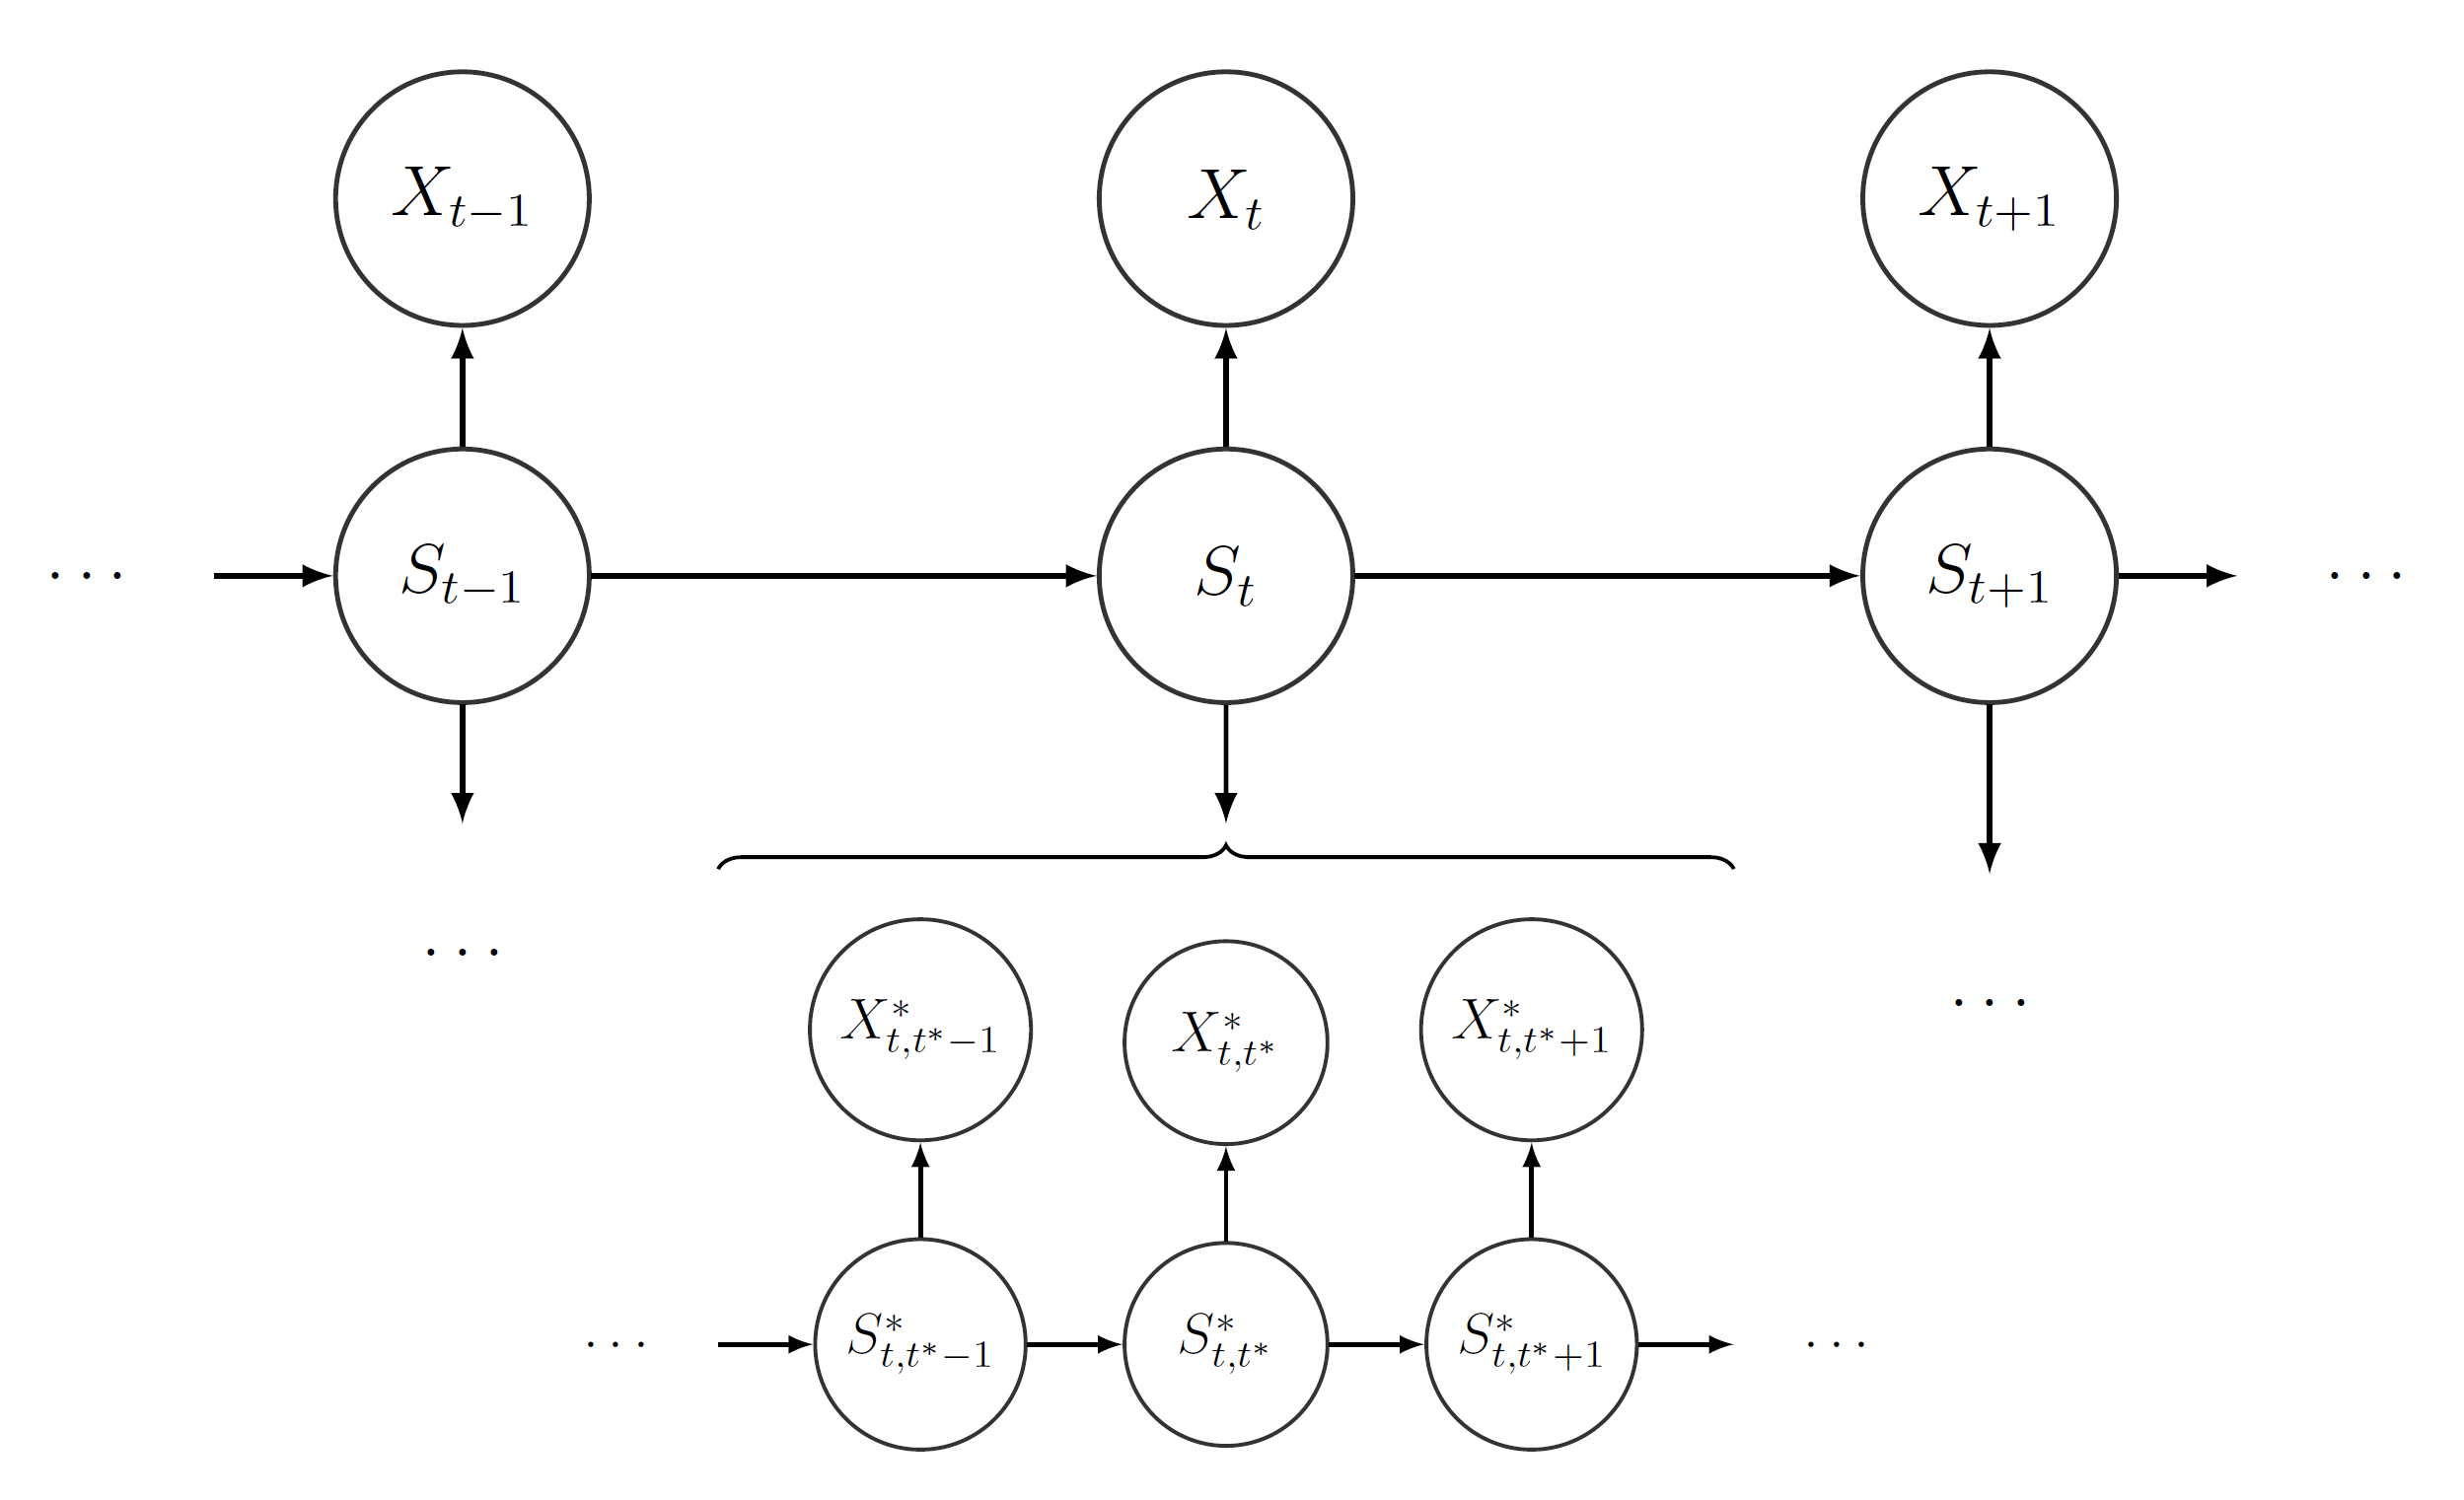
\includegraphics[scale = 0.6]{hhmm.png}
  \caption{Dependence structure of an HHMM.}
  \label{fig:hhmm}
\end{figure}

\section{Model specification} \label{sec:model_specification} %% Lennart

Model specification in the \pkg{fHMM} is done by specifying a named list of controls and passing it to the \fct{set\_controls} function. The function checks the specifications and returns an \class{fHMM\_controls} object which stores all specifications and thereby provides required information for other \pkg{fHMM} functionalities. In the following, we demonstrate example specifications that should help the user to tailor a hidden Markov model to their need. All possible specifications are documented in detail on the help page \code{help(set_controls, package = "fHMM")}.

Say that we want to fit an HMM to the closing prices of the Deutscher Aktienindex DAX \cite{jan92}. The data can be obtained from https://finance.yahoo.com/ or directly via the \fct{download\_data} function. The next section on data management introduces this function and lists all data requirements. For now, assume that our working directory contains the file \code{"dax.csv"}, which is in the correct format. Consider the following lines:

%
\begin{Schunk}
\begin{Sinput}
R> controls <- list(
+    states = 3,
+    sdds   = "t",
+    data   = list(file        = "dax.csv",
+                  date_column = "Date",
+                  data_column = "Close",
+                  logreturns  = TRUE)
+  )
R> controls <- set_controls(controls)
R> class(controls)
\end{Sinput}
\begin{Soutput}
[1] "fHMM_controls"
\end{Soutput}
\end{Schunk}
%

We specified a 3-state HMM (\code{states = 3}) with state-dependent t-distributions (\code{sdds = "t"}). The \code{data} element sets the path to the file (\code{file = "dax.csv"}), the file's column that contains the dates (\code{date_column = "Date"}) and the data (\code{date_column = "Close"}), and the command \code{logreturns = TRUE} that transforms the data to log-returns. The output of \fct{set\_controls} can then be passed to the estimation routine introduced in section \ref{sec:model_estimation}.

If the \code{data} element is not set, data will be simulated from the model specification. For example, the following specifies a 2-state HMM with state-dependent Gamma distributions, where the expectation values for state 1 and 2 are fixed to \code{0.5} and \code{2}, respectively. The model will be fitted to 500 data points (\code{horizon = 500}) simulated from this specification based on \code{runs = 50} randomly initialized numerical optimization of the model's log-likelihood function:

%
\begin{Schunk}
\begin{Sinput}
R> controls <- list(
+    states  = 2,
+    sdds    = "gamma(mu = 0.5|2)",
+    horizon = 500,
+    fit     = list(runs = 50)
+  )
R> set_controls(controls)
\end{Sinput}
\begin{Soutput}
fHMM controls:
* hierarchy: FALSE 
* data type: simulated 
* number of states: 2 
* sdds: gamma(mu = 0.5|2) 
* number of runs: 50  
\end{Soutput}
\end{Schunk}
%

The print method of the \class{fHMM\_controls} object summarizes the specification. Per default, the model has no hierarchy. To specify a hierarchical HMM, add \code{hierarchy = TRUE}. The rest is analogue, except that some parameters now can be specified for both hierarchies, where the first entry is for the coarse- and the second for the fine-scale, respectively:

%
\begin{Schunk}
\begin{Sinput}
R> controls <- list(
+    hierarchy = TRUE,
+    states    = c(3, 2),
+    sdds      = c("t(df = 1)", "t(df = Inf)"),
+    horizon   = c(100, 10)
+  )
R> set_controls(controls)
\end{Sinput}
\begin{Soutput}
fHMM controls:
* hierarchy: TRUE 
* data type: simulated 
* number of states: 3 2 
* sdds: t(df = 1) t(df = Inf) 
* number of runs: 100  
\end{Soutput}
\end{Schunk}
%

We specified an hierarchical HMM with \code{3} coarse-scale and \code{2} fine-scale states \code{states = c(3, 2)} and state-dependent t-distributions. The degrees of freedom are fixed to \code{-1} on the coarse-scale and \code{Inf} on the fine-scale (which results in a normal distribution).


\section{Data management} \label{sec:data_management} %% Lennart

Empirical data for modeling must be provided as a comma-separated values (CSV) file and its path must be specified in \fct{set\_controls}, see the previous section. We recommend to use the data provided by https://finance.yahoo.com/. The \pkg{fHMM} package includes the convenience function \fct{download\_data} for downloading daily stock data directly from the website in the required format. The function call is \code{download\_data(symbol, from, to, file)}, where

- \code{symbol} is the stock's symbol that has to match the official symbol on https://finance.yahoo.com,

- \code{from} and \code{to} define the time interval (in format \code{"YYYY-MM-DD"}),

- \code{file} is the name of the file where the .csv-file is saved. Per default, it is saved in the current working directory under the name \code{<symbol>.csv}.

For example, the call

%
\begin{Schunk}
\begin{Sinput}
R> download_data(symbol = "^GDAXI", from = "2000-01-01", to = Sys.Date())
\end{Sinput}
\begin{Soutput}
Download successful.
* symbol: ^GDAXI 
* from: 2000-01-03 
* to: 2022-04-04 
* path: C:\Users\Lennart\Projekte\fHMM\jss\^GDAXI.csv
\end{Soutput}
\end{Schunk}
%

downloads the 21st century daily data of the DAX into the current working directory.

The \pkg{fHMM} package already includes two data sets of the Deutscher Aktienindex DAX and the VW stock for demonstration purpose that can be accessed as follows:

%
\begin{Schunk}
\begin{Sinput}
R> system.file("extdata", "dax.csv", package = "fHMM")
R> system.file("extdata", "vw.csv", package = "fHMM")
\end{Sinput}
\end{Schunk}
%

The \code{prepare\_data} function prepares the data based on the \class{fHMM\_controls} specifications and returns an \class{fHMM\_data} object that can be passed to the \fct{fit\_model} function for model fitting, see the next section:

%
\begin{Schunk}
\begin{Sinput}
R> controls <- list(
+    states = 3,
+    sdds   = "t",
+    data   = list(file        = system.file("extdata", "dax.csv", package = "fHMM"),
+                  date_column = "Date",
+                  data_column = "Close",
+                  from        = "2000-01-01",
+                  to          = "2021-12-31",
+                  logreturns  = TRUE),
+    fit    = list(runs        = 100)
+  )
R> controls <- set_controls(controls)
R> data <- prepare_data(controls)
R> class(data)
\end{Sinput}
\begin{Soutput}
[1] "fHMM_data"
\end{Soutput}
\end{Schunk}
%

The \class{fHMM\_data} object has a \fct{summary} method for a quick data overview:

%
\begin{Schunk}
\begin{Sinput}
R> summary(data)
\end{Sinput}
\begin{Soutput}
Summary of fHMM empirical data
* number of observations: 5626 
* data source: dax.csv 
* date column: Date 
* log returns: TRUE 
\end{Soutput}
\end{Schunk}
%

Additionally, the data can be visualized via the \fct{plot} method, where historical events can be highlighted by specifying a named list \code{events} with elements \code{dates} (a vector of dates) and \code{labels} (a vector of labels for the events) and passing it to the plot method, for example:

%
\begin{Schunk}
\begin{Sinput}
R> events <- fHMM_events(
+    list(
+      dates = c("2001-09-11", "2008-09-15", "2020-01-27"),
+      labels = c("9/11 terrorist attack", "Bankruptcy of Lehman Brothers", 
+                 "First COVID-19 case in Germany")
+      )
+    )
R> plot(data, events = events)
\end{Sinput}
\end{Schunk}
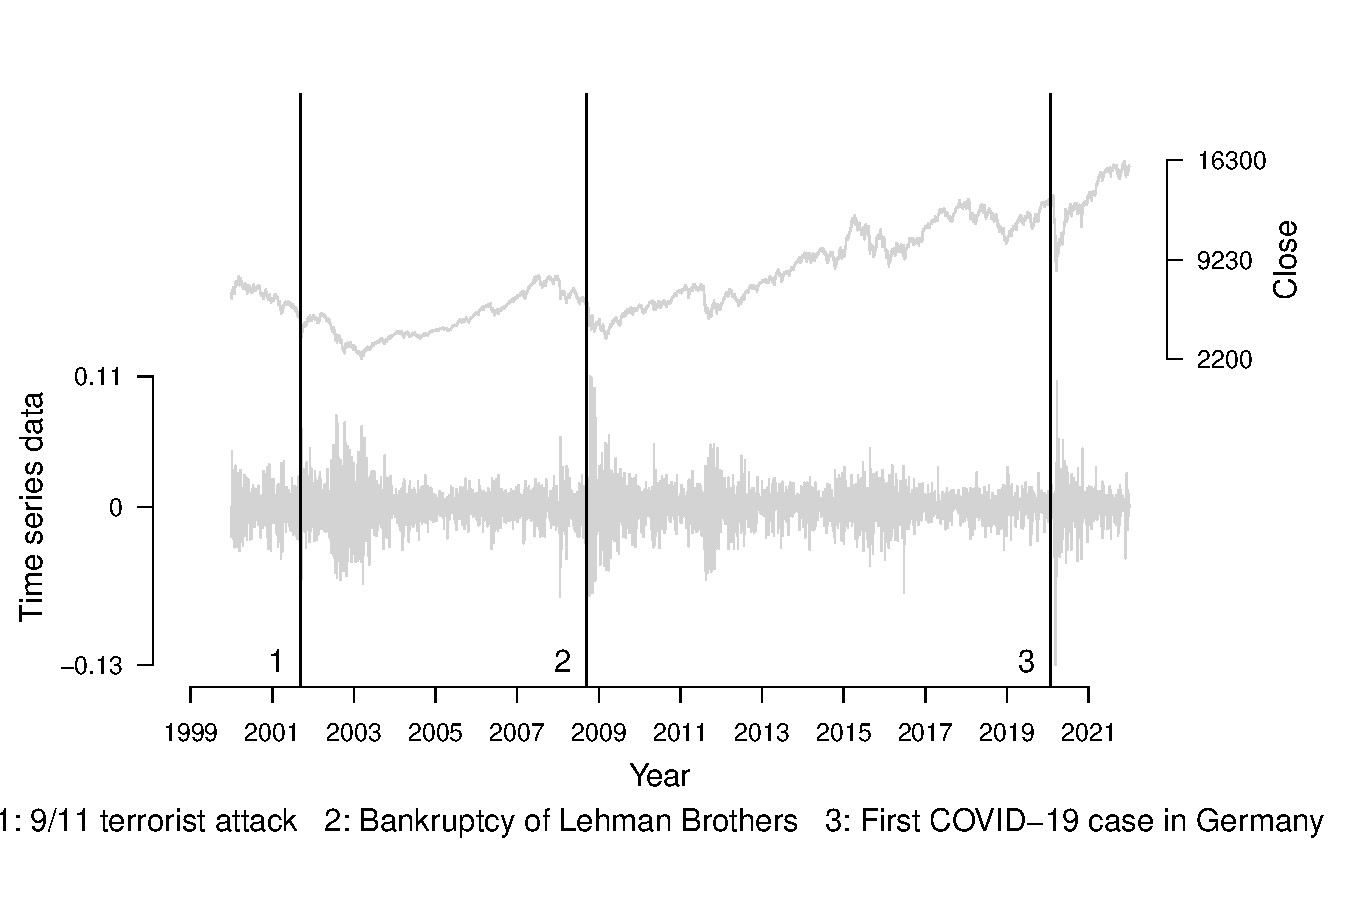
\includegraphics{fhmm_oelschlaeger_adam_michels-ts}
%

As mentioned in the previous section, if the \code{data} parameter in the model's \code{controls} is unspecified, the model is fitted to simulated data from the model specification. This can be useful for testing the functionality or conducting simulation experiments. True model parameters can be specified by defining an \class{fHMM\_parameters}-object via the \fct{fHMM\_parameters} function and passing it to \fct{prepare\_data}.

An example: In the previous section, we specified the following \code{controls}:

%
\begin{Schunk}
\begin{Sinput}
R> controls <- list(
+    states  = 2,
+    sdds    = "gamma(mu = 0.5|2)",
+    horizon = 500,
+    fit     = list(runs = 50)
+  )
R> controls <- set_controls(controls)
\end{Sinput}
\end{Schunk}
%

The means of the Gamma distributions in the two states are fixed to \code{0.5} and \code{2}. With the following lines, we specify the transition probability matrix \code{Gamma} and the standard deviations \code{sigmas}:

%
\begin{Schunk}
\begin{Sinput}
R> pars <- fHMM_parameters(
+    controls = controls, Gamma = matrix(c(0.9,0.2,0.1,0.8), nrow = 2), 
+    sigmas = c(0.1,0.5)
+  )
R> class(pars)
\end{Sinput}
\begin{Soutput}
[1] "fHMM_parameters"
\end{Soutput}
\end{Schunk}
%

Submitting the \class{fHMM\_parameters} object together with \code{controls} to \fct{prepare\_data} creates the (simulated) \class{fHMM\_data} object:

%
\begin{Schunk}
\begin{Sinput}
R> data <- prepare_data(controls, true_parameters = pars, seed = 1)
R> plot(data)
\end{Sinput}
\end{Schunk}
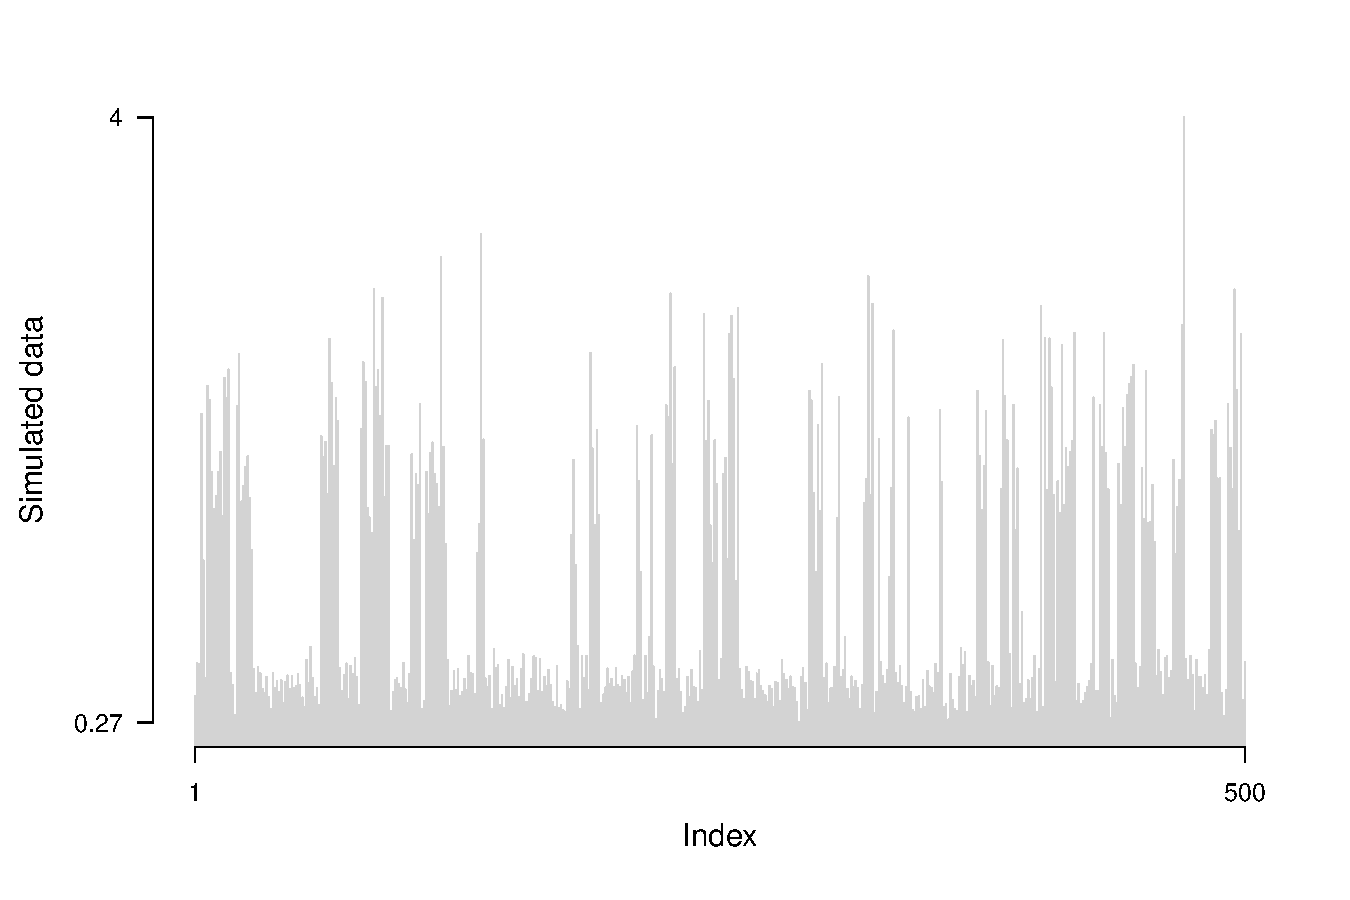
\includegraphics{fhmm_oelschlaeger_adam_michels-simdata}
%

The \class{fHMM\_data} object can now be passed to the \fct{fit\_model} function for model estimation, which is explained in the next section.

\section{Model estimation} \label{sec:model_estimation} %% Timo + Lennart

The \pkg{fHMM} package fits a hidden Markov model via the maximum-likelihood method, i.e.\ by numerically maximizing the likelihood function. Deriving the likelihood function of an hidden Markov model is part of the hierarchical case, hence the following only discusses the general case.

An HHMM can be treated as an HMM with two conditionally independent data streams; the coarse-scale observations on the one hand and the corresponding chunk of fine-scale observations connected to a fine-scale HMM on the other hand. To derive the likelihood of an HHMM, we start by computing the likelihood of each chunk of fine-scale observations being generated by each fine-scale HMM. 

To fit the $i$-th fine-scale HMM, with model parameters $\theta^{*(i)}=(\delta^{*(i)}, \Gamma^{*(i)},(f^{*(i,k)})_k)$ to the $t$-th chunk of fine-scale observations, which is denoted by $(X_{t,t^*})_{t^*}$, we consider the fine-scale forward probabilities 
\begin{align*}
\alpha^{*(i)}_{k,t^*}=f^{*(i)}(X^*_{t,1},\dots,X^*_{t,t^*}, S^*_{t,t^*}=k),
\end{align*}
where $t^*=1,\dots,T^*$ and $k=1,\dots,N^*$. Using the fine-scale forward probabilities, the fine-scale likelihoods can be obtained from the law of total probability as
\begin{align*}
\mathcal{L}^\text{HMM}(\theta^{*(i)}\mid (X^*_{t,t^*})_{t^*})=\sum_{k=1}^{N^*}\alpha^{*(i)}_{k,T^*}.
\end{align*}
The forward probabilities can be calculated in a recursively as
\begin{align*}
\alpha^{*(i)}_{k,1} &= \delta^{*(i)}_k f^{*(i,k)}(X^*_{t,1}), \\
\alpha^{*(i)}_{k,t^*} &= f^{*(i,k)}(X^*_{t,t^*})\sum_{j=1}^{N^*}\gamma^{*(i)}_{jk}\alpha^{*(i)}_{j,t^*-1}, \quad t^*=2,\dots,T^*.
\end{align*}

The transition from the likelihood function of an HMM to the likelihood function of an HHMM is straightforward: Consider the coarse-scale forward probabilities
\begin{align*}
\alpha_{i,t}=f(X_1,\dots,X_t,(X^*_{1,t^*})_{t^*},\dots,(X^*_{t,t^*})_{t^*}, S_t=i),
\end{align*}
where $t=1,\dots,T$ and $i=1,\dots,N$. The likelihood function of the HHMM results as
\begin{align*}
\mathcal{L}^\text{HHMM}(\theta,(\theta^{*(i)})_i\mid (X_t)_t,((X^*_{t,t^*})_{t^*})_t)=\sum_{i=1}^{N}\alpha_{i,T}.
\end{align*}
The coarse-scale forward probabilities can be calculated similarly by applying the recursive scheme
\begin{align*}
\alpha_{i,1} &= \delta_i \mathcal{L}^\text{HMM}(\theta^{*(i)}\mid (X^*_{1,t^*})_{t^*})f^{(i)}(X_1), \\
\alpha_{i,t} &= \mathcal{L}^\text{HMM}(\theta^{*(i)}\mid (X^*_{t,t^*})_{t^*}) f^{(i)}(X_t)\sum_{j=1}^{N}\gamma_{ji}\alpha_{j,t-1}, \quad t=2,\dots,T.
\end{align*}

To account for parameter constraints associated with the transition probabilities (and potentially the parameters of the state-dependent distributions), we use parameter transformations. To ensure that the entries of the t.p.m.s fulfill non-negativity and the unity condition, we estimate unconstrained values $(\eta_{ij})_{i\neq j}$ for the non-diagonal entries of $\Gamma$ and derive the probabilities using the multinomial logit link
\begin{align*}
\gamma_{ij}=\frac{\exp[\eta_{ij}]}{1+\sum_{k\neq i}\exp[\eta_{ik}]},~i\neq j
\end{align*}
rather than estimating the probabilities $(\gamma_{ij})_{i,j}$ directly. The diagonal entries result from the unity condition as
\begin{align*}
\gamma_{ii}=1-\sum_{j\neq i}\gamma_{ij}.
\end{align*}
Furthermore, variances are strictly positive, which can be achieved by applying an exponential transformation to the unconstrained estimator.

When numerically maximizing the likelihood using some Newton-Raphson-type method, we often face numerical under- or overflow, which can be addressed by maximizing the logarithm of the likelihood and incorporating constants in a conducive way (see \cite{zuc16} and \cite{oel21} for details).

As the likelihood is maximized with respect to a relatively large number of parameters, the obtained maximum can be a local rather than the global one. To avoid this problem, it is recommended to run the maximization multiple times from different, possibly randomly selected starting points, and to choose the model that corresponds to the highest likelihood (see \cite{zuc16} and \cite{oel21} for details).

For illustration, we fit a 3-state HMM with state-dependent t-distributions to the DAX data. We use the same specification as in the previous section:

%
\begin{Schunk}
\begin{Sinput}
R> controls <- list(
+    states = 3,
+    sdds   = "t",
+    data   = list(file        = system.file("extdata", "dax.csv", package = "fHMM"),
+                  date_column = "Date",
+                  data_column = "Close",
+                  from        = "2000-01-01",
+                  to          = "2021-12-31",
+                  logreturns  = TRUE),
+    fit    = list("runs" = 100)
+  )
R> controls <- set_controls(controls)
R> data <- prepare_data(controls)
\end{Sinput}
\end{Schunk}
%

The \class{data} object can be directly passed to the \fct{fit\_model} function that numerically maximizes the model's (log-) likelihood function \code{runs = 100} times. For convenience, the \class{controls} object is saved in \class{data} and does not need to be submitted to \fct{fit\_model}. The numerical maximization runs can be parallelized by setting the \code{ncluster} argument. Setting \code{ncluster = 1} avoids any dependency on packages that provide clustering.

%
\begin{Schunk}
\begin{Sinput}
R> dax_model_3t <- fit_model(data, seed = 1, verbose = FALSE)
\end{Sinput}
\end{Schunk}
%

The estimated model is saved in the \pkg{fHMM} package and can be accessed as follows:

%
\begin{Schunk}
\begin{Sinput}
R> data(dax_model_3t)
\end{Sinput}
\end{Schunk}
%

The \fct{coef} method returns a data frame of the estimated model coefficients:

%
\begin{Schunk}
\begin{Sinput}
R> coef(dax_model_3t)
\end{Sinput}
\begin{Soutput}
                     lb      estimate           ub
Gamma_2.1  2.790298e-03  5.145659e-03 9.428763e-03
Gamma_3.1            NA  1.499800e-69           NA
Gamma_1.2            NA  1.740120e-02           NA
Gamma_3.2            NA  2.640840e-02           NA
Gamma_1.3            NA  1.972455e-64           NA
Gamma_2.3  1.393931e-02  2.170081e-02 3.356866e-02
mu_1      -3.725797e-03 -1.673721e-03 3.783550e-04
mu_2      -7.968519e-04 -2.517697e-04 2.933126e-04
mu_3       9.609845e-04  1.268698e-03 1.576411e-03
sigma_1    2.329705e-02  2.562672e-02 2.818935e-02
sigma_2    1.269102e-02  1.323830e-02 1.380917e-02
sigma_3    5.332188e-03  5.774416e-03 6.253320e-03
df_1       5.501359e+00  1.064328e+01 2.059118e+01
df_2       4.957714e+75  4.957714e+75 4.957714e+75
df_3       3.964123e+00  5.272141e+00 7.011757e+00
\end{Soutput}
\end{Schunk}
%

The estimated state-dependent distributions can be plotted as follows:

%
\begin{Schunk}
\begin{Sinput}
R> plot(dax_model_3t, plot_type = "sdds")
\end{Sinput}
\end{Schunk}
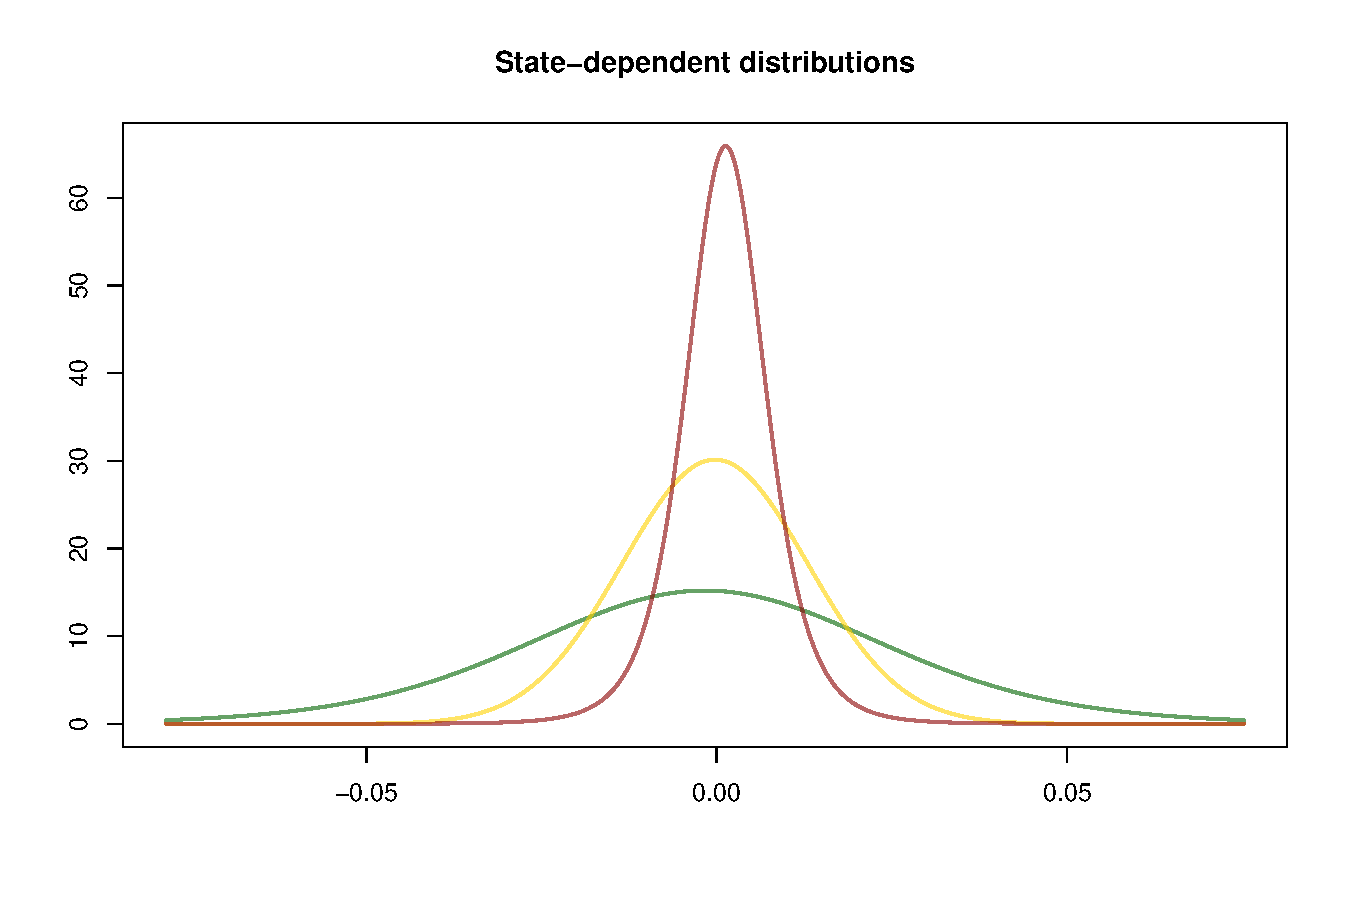
\includegraphics{fhmm_oelschlaeger_adam_michels-sdds}
%

As mentioned above, the HMM likelihood function is prone to local optima. This effect can be visualized by plotting the log-likelihood value in the different optimization runs, where the best run is marked in red:

%
\begin{Schunk}
\begin{Sinput}
R> plot(dax_model_3t, plot_type = "ll")
\end{Sinput}
\end{Schunk}
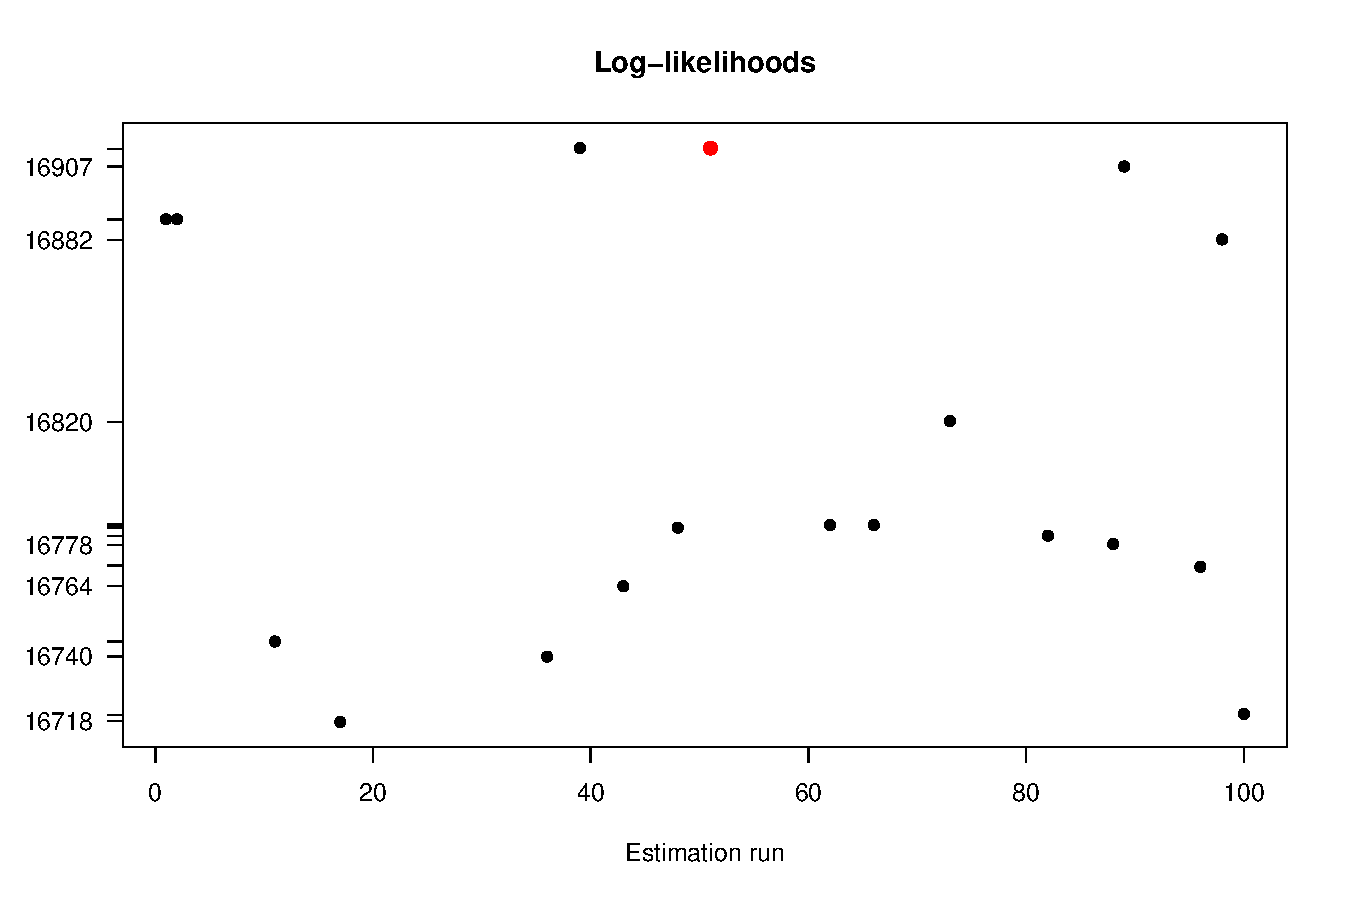
\includegraphics{fhmm_oelschlaeger_adam_michels-ll}
%

The package also includes an hierarchical HMM with the following specification:

%
\begin{Schunk}
\begin{Sinput}
R> data(dax_vw_model)
R> plot(dax_vw_model, plot_type = "sdds")
\end{Sinput}
\end{Schunk}
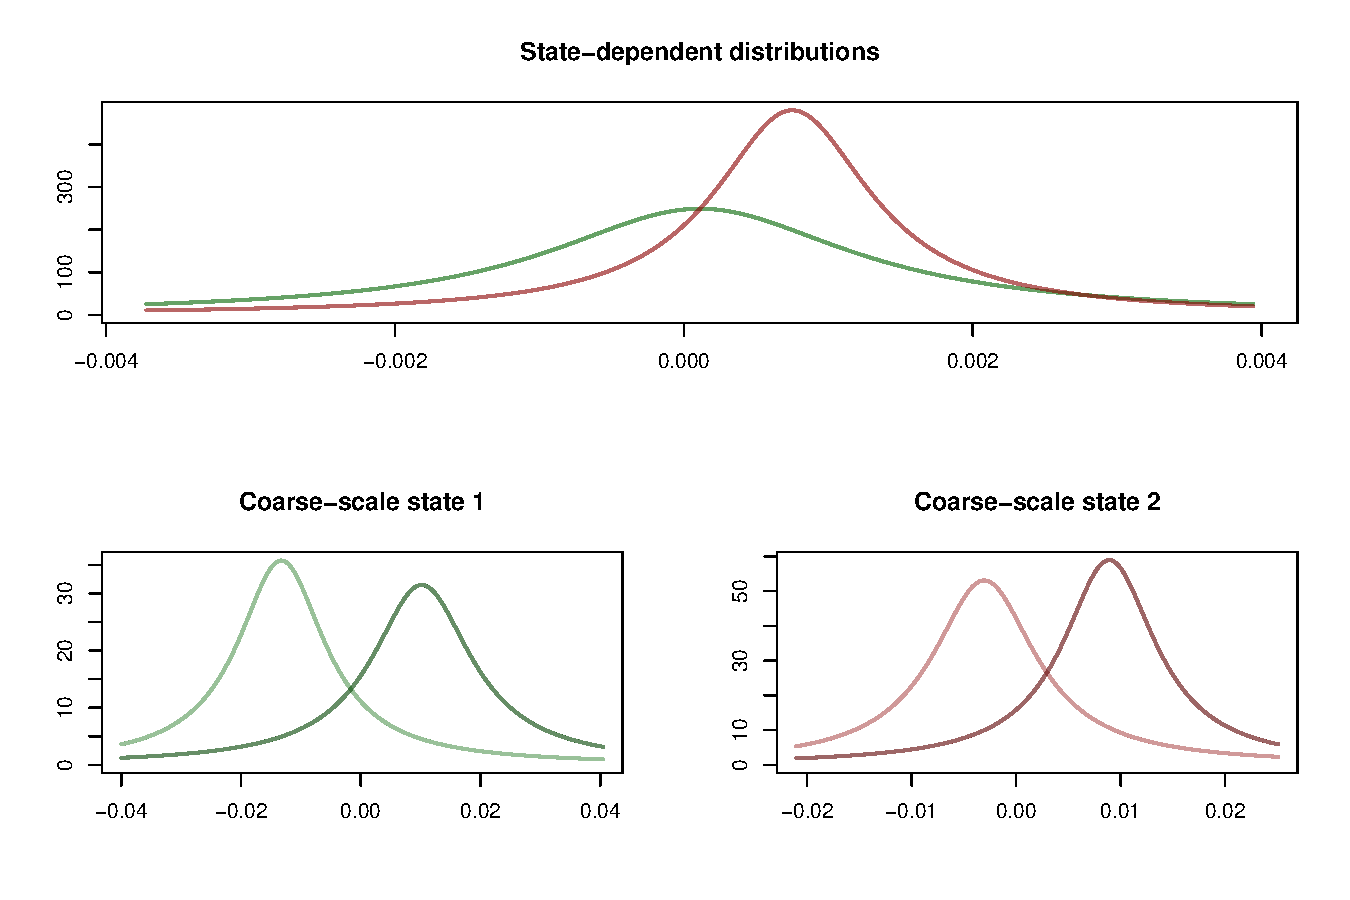
\includegraphics{fhmm_oelschlaeger_adam_michels-hhmm_model}
%


\section{State decoding and prediciton} \label{sec:state_decoding_and_prediction} %% Rouven + Lennart

For financial markets, it is of special interest to infer the underlying (hidden) states in order to gain insight about the actual market situation. Decoding a full time series $S_1, \ldots, S_T$ is called \textbf{global decoding}. Hereby, we aim to find the most likely trajectory of hidden states under the estimated model. 
Global decoding can be accomplished by using the so-called Viterbi algorithm which is a recursive scheme enabling to find the global maximum without being confronted with huge computational costs. To this end, we follow \cite{zuc16} and define
$$\zeta_{1i} = Pr(S_1 = i, X_1 = x_1) = \delta_i p_i(x_1)$$ 
for $i = 1, \ldots, N$ and for the following $t = 2, \ldots, T$
$$\zeta_{ti} = \operatorname*{max}_{s_1, \ldots, s_{t-1}} Pr(S_{t-1} = s_{t-1}, S_t = i, X_t = x_t).$$ 
Then, the trajectory of most likely states $i_1, \ldots, i_T$ can be calculated recursively from
$$i_T = \operatorname*{argmax}_{i = 1, \ldots, N} \zeta_{Ti}$$ and for the following $t = T-1, \ldots, 1$ from
$$i_t = \operatorname*{argmax}_{i = 1, \ldots, N} (\zeta_{ti} \gamma_{i, i_{t+1}}).$$

Transferring the state decoding to HHMMs is straightforward: at first the coarse-scale state process must be decoded. Afterwards, by using this information the fine-scale state process can be decoded, see \cite{ada19}.

We revisit the DAX model of the vignette on model estimation:

%
\begin{Schunk}
\begin{Sinput}
R> data(dax_model_3t)
\end{Sinput}
\end{Schunk}
%

The underlying states can be decoded via the \fct{decode\_states} function:

%
\begin{Schunk}
\begin{Sinput}
R> dax_model_3t <- decode_states(dax_model_3t)
\end{Sinput}
\end{Schunk}
%

We now can visualize the decoded time series:

%
\begin{Schunk}
\begin{Sinput}
R> plot(dax_model_3t)
\end{Sinput}
\end{Schunk}
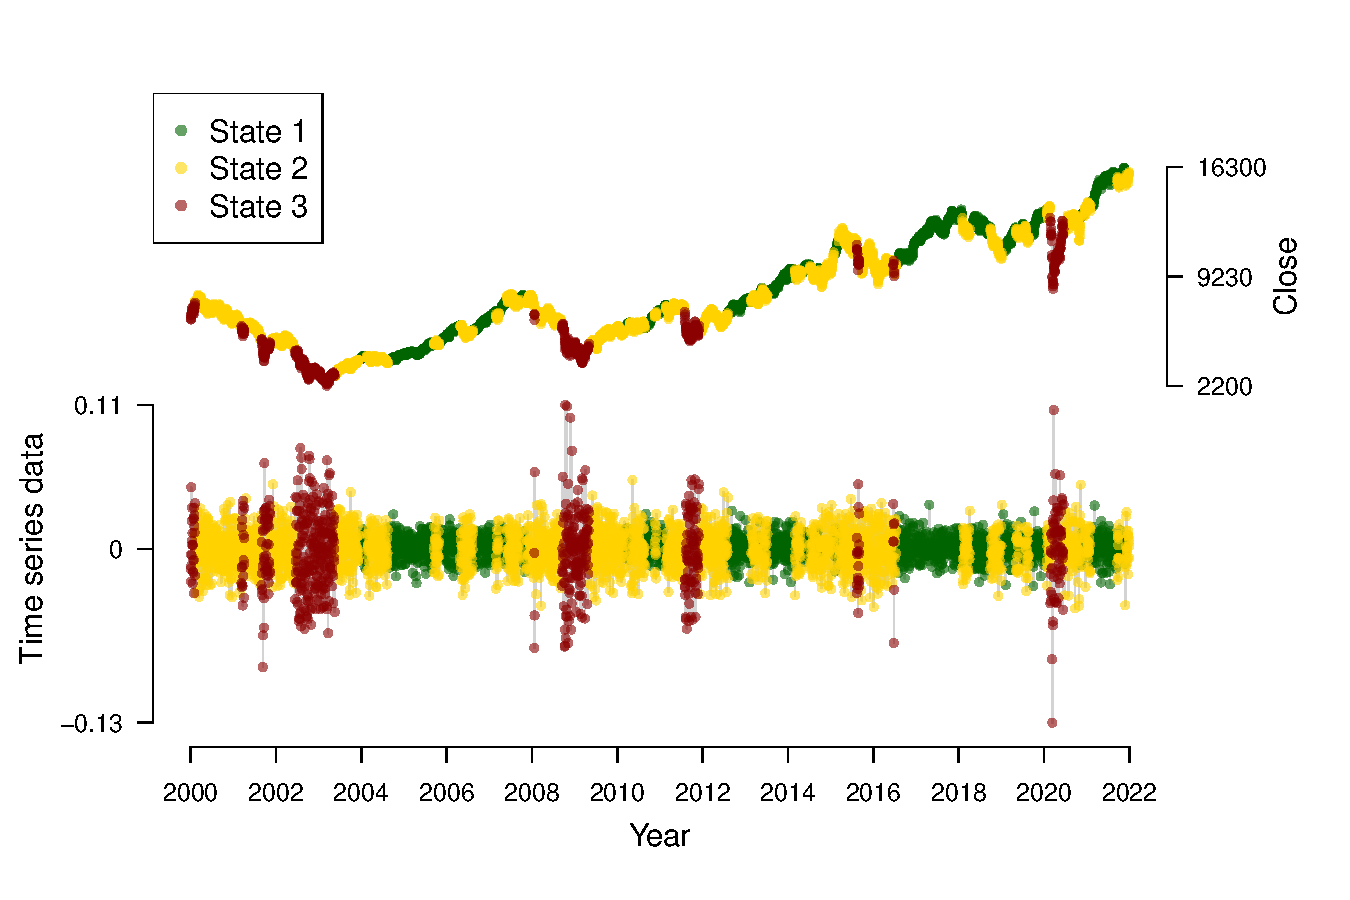
\includegraphics{fhmm_oelschlaeger_adam_michels-dec_ts}
%

Mind that the model is invariant to permutations of the state labels. Therefore, \pkg{fHMM} provides the option to switch labels after decoding via the \fct{reorder\_states} function, for example:

%
\begin{Schunk}
\begin{Sinput}
R> dax_model_3t <- reorder_states(dax_model_3t, 3:1)
\end{Sinput}
\end{Schunk}
%

Having decoded the underlying states, it is possible to compute the state probabilities of next observations. Based on these probabilities and in combination with the estimated state-dependent distributions, next observations can be predicted, compare \cite{zuc16}:

%
\begin{Schunk}
\begin{Sinput}
R> predict(dax_model_3t, ahead = 10)
\end{Sinput}
\begin{Soutput}
      state_1   state_2     state_3          lb
1  0.02170081 0.9731535 0.005145659 -0.02190377
2  0.04224595 0.9476904 0.010063634 -0.02178845
3  0.06169596 0.9235390 0.014765007 -0.02168046
4  0.08010821 0.9006315 0.019260295 -0.02157939
5  0.09753712 0.8789034 0.023559485 -0.02148485
6  0.11403424 0.8582937 0.027672059 -0.02139648
7  0.12964845 0.8387445 0.031607018 -0.02131393
8  0.14442608 0.8202010 0.035372911 -0.02123689
9  0.15841104 0.8026111 0.038977855 -0.02116504
10 0.17164498 0.7859255 0.042429556 -0.02109809
        estimate         ub
1  -2.260912e-04 0.02145158
2  -2.018461e-04 0.02138476
3  -1.789581e-04 0.02132255
4  -1.573549e-04 0.02126468
5  -1.369681e-04 0.02121091
6  -1.177326e-04 0.02116101
7  -9.958705e-05 0.02111476
8  -8.247306e-05 0.02107194
9  -6.633542e-05 0.02103237
10 -5.112181e-05 0.02099584
\end{Soutput}
\end{Schunk}
%




\section{Model checking} \label{sec:model_checking} %% Timo + Lennart

Analyzing pseudo-residuals allows us to check whether the fitted model describes the data well. Since the observations are explained by different distributions (depending on the active state), this cannot be done by analyzing standard residuals. To transform all observations on a common scale, we proceed as follows: If $X_t$ has the invertible distribution function $F_{X_t}$, then

\begin{align*}
Z_t=\Phi^{-1}(F_{X_t} (X_t))
\end{align*}

is standard normally distributed, where $\Phi$ denotes the cumulative distribution function of the standard normal distribution. The observations, $(X_t)_t$, are modeled well if the so-called pseudo-residuals, $(Z_t)_t$, are approximately standard normally distributed, which can be visually assessed using quantile-quantile plots or further investigated using statistical tests such as the Jarque-Bera test \cite{zuc16}. 

For HHMMs, we first decode the coarse-scale state process using the Viterbi algorithm. Subsequently, we assign each coarse-scale observation its distribution function under the fitted model and perform the transformation described above. Using the Viterbi-decoded coarse-scale states, we then treat the fine-scale observations analogously.

In \pkg{fHMM}, pseudo-residuals can be computed via the \fct{compute\_residuals} function, provided that the states have been decoded beforehand.

We revisit the DAX example:

%
\begin{Schunk}
\begin{Sinput}
R> data(dax_model_3t)
\end{Sinput}
\end{Schunk}
%

The following line computes the residuals and saves them into the \code{model} object:

%
\begin{Schunk}
\begin{Sinput}
R> dax_model_3t <- compute_residuals(dax_model_3t)
\end{Sinput}
\end{Schunk}
%

The residuals can be visualized as follows:

%
\begin{Schunk}
\begin{Sinput}
R> plot(dax_model_3t, plot_type = "pr")
\end{Sinput}
\end{Schunk}
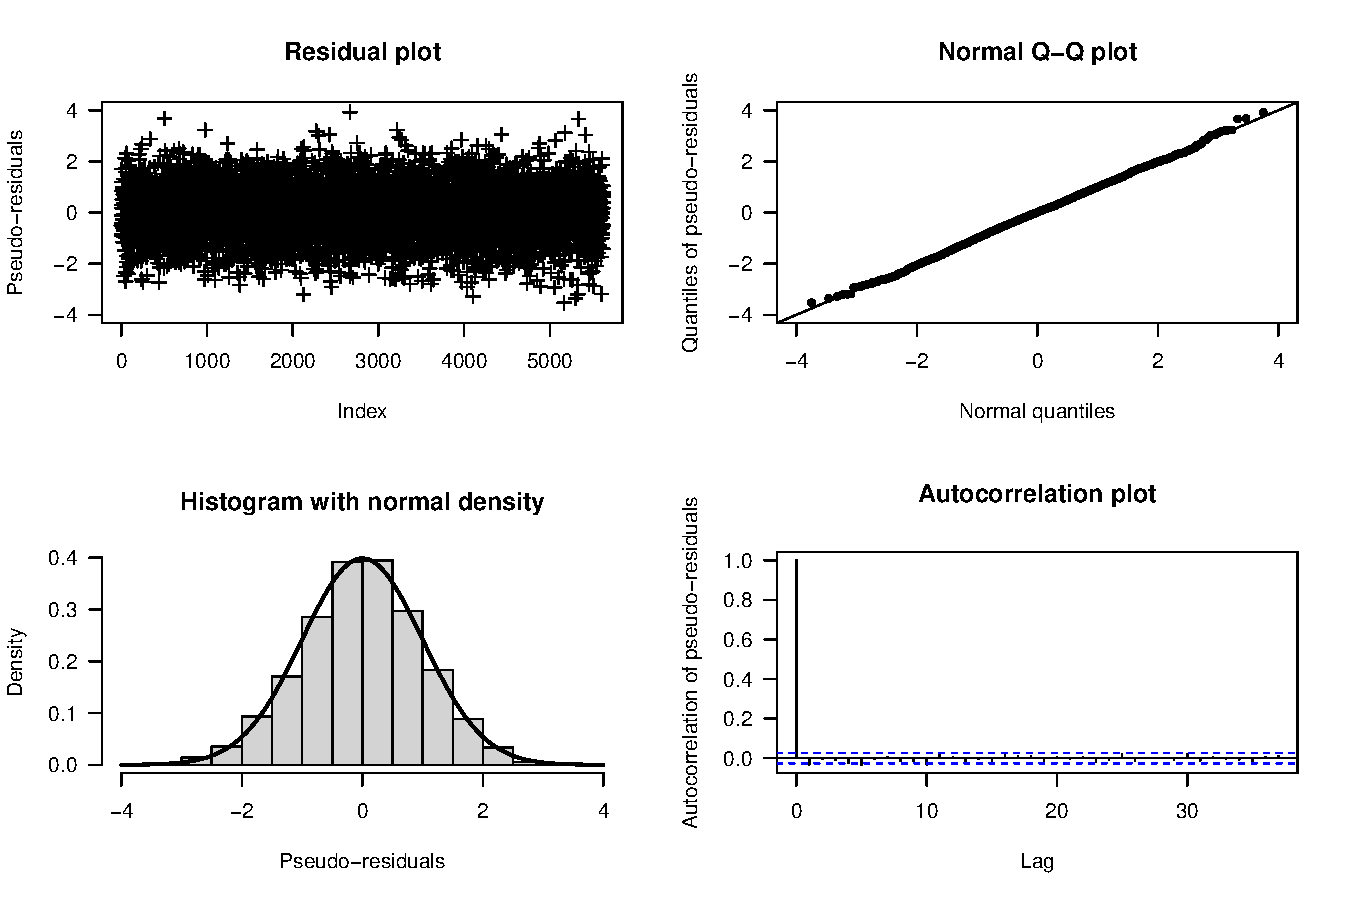
\includegraphics{fhmm_oelschlaeger_adam_michels-residuals}
%

For additional normality tests, the residuals can be extracted from the \code{model} object. The following lines exemplary perform a Jarque-Bera test \cite{jar87}:

%
\begin{Schunk}
\begin{Sinput}
R> res <- dax_model_3t$residuals
R> tseries::jarque.bera.test(res)
\end{Sinput}
\begin{Soutput}
	Jarque Bera Test

data:  res
X-squared = 2.6558, df = 2, p-value = 0.265
\end{Soutput}
\end{Schunk}
%

\section{Model selection} \label{sec:model_selection} %% Timo + Lennart

Model selection involves the choice of a family for the state-dependent distribution and the selection of the number of states. Common model selection tools are information criteria, such as the Akaike information criterion (AIC) or the Bayesian information criterion (BIC), both of which aim at finding a compromise between model fit and model complexity.

The AIC is defined as
\begin{align*}
\text{AIC} = - 2 \log (\mathcal{L}^\text{(H)HMM}(\theta,(\theta^{*(i)})_i\mid (X_t)_t,((X^*_{t,t^*})_{t^*})_t)) + 2 p,
\end{align*}
where $p$ denotes the number of parameters, while the BIC is defined as
\begin{align*}
\text{BIC} = - 2 \log (\mathcal{L}^\text{(H)HMM}(\theta,(\theta^{*(i)})_i\mid (X_t)_t,((X^*_{t,t^*})_{t^*})_t)) + \log(T) p,
\end{align*}
where $T$ is the number of observations.

In practice, however, information criteria often favor overly complex models. Real data typically exhibit more structure than can actually be captured by the model. This can be the case if the true state-dependent distributions are too complex to be fully modeled by some (rather simple) parametric distribution, or if certain temporal patterns are neglected in the model formulation. Additional states may be able to capture this structure, which can lead to an increased goodness of fit that outweighs the higher model complexity. However, as models with too many states are difficult to interpret and are therefore often not desired, information criteria should be treaten with some caution and only considered as a rough guidance. For an in-depth discussion of pitfalls, practical challenges, and pragmatic solutions regarding model selection, see \cite{poh17}.

The \pkg{fHMM} package provides a convenient tool for comparing different models via the \fct{compare\_models} function. The models (arbitrarily many) can be directly passed to the \fct{compare\_models} function that returns an overview of the above model selection criteria. Below, we compare a 2-state HMM with normal state-dependent distributions with a 3-state HMM with state-dependent t-distributions for the DAX data, where the more complex model is clearly preffered:

%
\begin{Schunk}
\begin{Sinput}
R> data(dax_model_2n)
R> data(dax_model_3t)
R> compare_models(dax_model_2n, dax_model_3t)
\end{Sinput}
\begin{Soutput}
             parameters log-likelihood       AIC       BIC
dax_model_2n          6       16681.98 -33351.96 -33312.15
dax_model_3t         15       16913.33 -33796.65 -33697.13
\end{Soutput}
\end{Schunk}
%


%% -- Summary/conclusions/discussion -------------------------------------------

\section{Conclusions} \label{sec:conclusion}

The \pkg{fHMM} package intends to make the estimation of hidden Markov models for financial data available to practitioners in a user-friendly way. It contains functionality for data management, model fitting, state decoding, model checking, model selection, and methods for visualization. The hierarchical model extension is included for modeling trends on two temporal resolutions. 

%% -- Optional special unnumbered sections -------------------------------------

\section*{Computational details}

The results in this paper were obtained using
\proglang{R}~4.1.2 with the
\pkg{fHMM}~1.0.0 package. \proglang{R} itself
and all packages used are available from the Comprehensive
\proglang{R} Archive Network (CRAN) at \url{https://CRAN.R-project.org/}.


% \section*{Acknowledgments}

%% -- Bibliography -------------------------------------------------------------
%% - References need to be provided in a .bib BibTeX database.
%% - All references should be made with \cite, \citet, \citep, \citealp etc.
%%   (and never hard-coded). See the FAQ for details.
%% - JSS-specific markup (\proglang, \pkg, \code) should be used in the .bib.
%% - Titles in the .bib should be in title case.
%% - Journal titles should not be abbreviated and in title case.
%% - DOIs should be included where available.
%% - Software should be properly cited as well.

\bibliography{ref}


%% -- Appendix (if any) --------------------------------------------------------
%% - After the bibliography with page break.
%% - With proper section titles and _not_ just "Appendix".
% 
% \newpage
% 
% \begin{appendix}
% 
% \section{Installation} \label{app:installation}
% 
% \end{appendix}
% 
%% -----------------------------------------------------------------------------


\end{document}
